\section{Datum}
\subsection{Pengertian DATUM}

Datum reference surface atau geodetik atau georeferensi adalah parameter sebagai referensi untuk mendefinisikan geometri Bumi ellipsoid. Datum geodetik diukur menggunakan metode manual agar lebih akurat lagi menggunakan satelit.

Dibawah ini merupakan Jenis geodetik menurut metodenya :
\begin{enumerate}
\item Datum horizontal adalah datum yang digunakan untuk pemetaan horisontal. Dengan teknologi yang lebih maju, kini muncul tren penggunaan datum horizontal dari koordinat geosentris global sebagai penggganti datum lokal atau regional.
\begin{figure}[htbp]
		\centering
		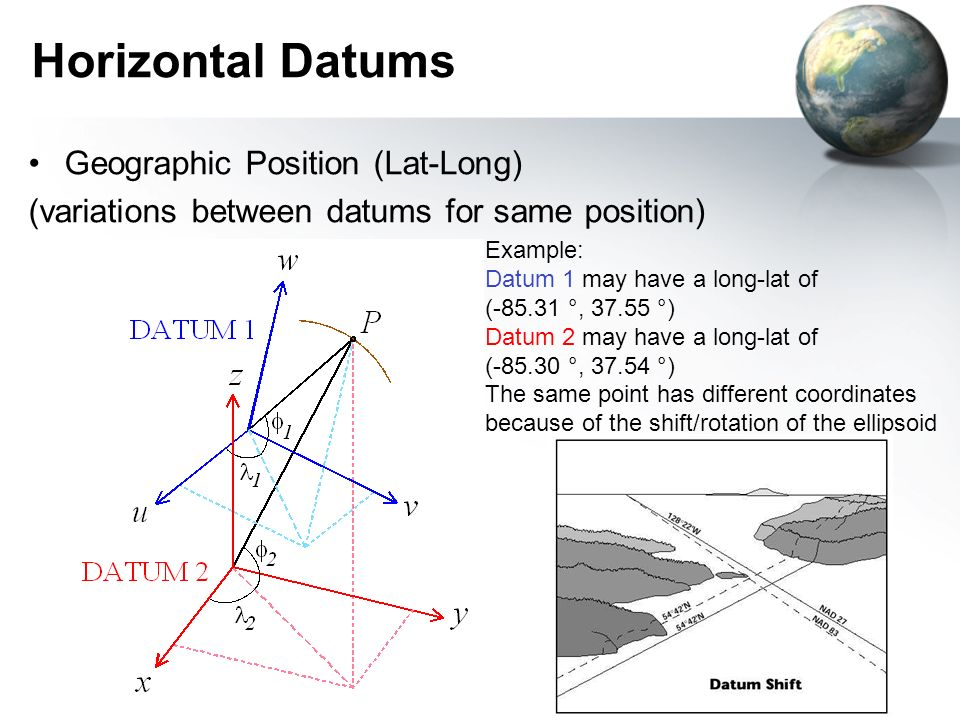
\includegraphics[width=0.75\textwidth]{pictures/datum_horizontal.jpg}
		\caption{Datum Horizontal (Sumber : https://www.slideshare.net/AeroMetri)}
		\label{Datum Horizontal}
		\end{figure}	

\item Datum vertikal adalah sistem referensi untuk ortometris medan tinggi. Datum vertikal digunakan untuk mewakili ketinggian atau kedalaman informasi. Biasanya bidang referensi yang digunakan untuk ortometris sistem tinggi adalah geoid.
\begin{figure}[htbp]
		\centering
		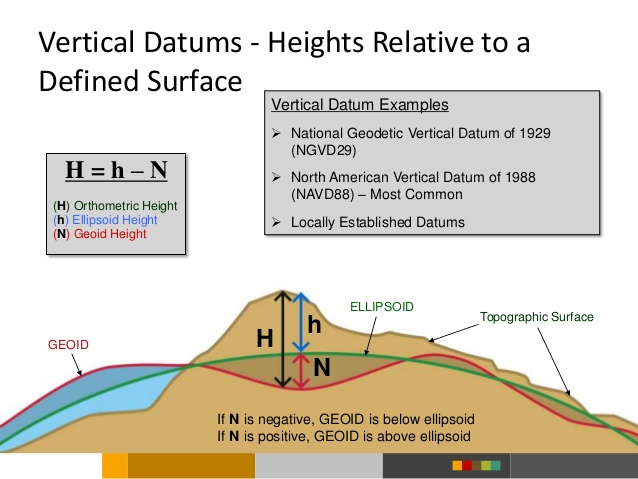
\includegraphics[width=0.75\textwidth]{pictures/vertical_datum.jpg}
		\caption{Datum Vertikal (Sumber : Map Projections and Coordinate Systems 2014)}
		\label{Datum Vertikal}
		\end{figure}	
\end{enumerate}

Sedangkan menurut jenisnya datum geodetik menurut luas areanya :
\begin{enumerate}
\item Datum geodetik lokal adalah bentuk geoid yang paling cocok pada area yang tidak terlalu besar. Sampel datum lokal di Indonesia antara lain: Genoek, datum Monconglowe datum, di 74 (Datum Indonesia 1974), dan dengan 95 (Datum Geodetik Indonesia 1995).
\begin{figure}[htbp]
		\centering
		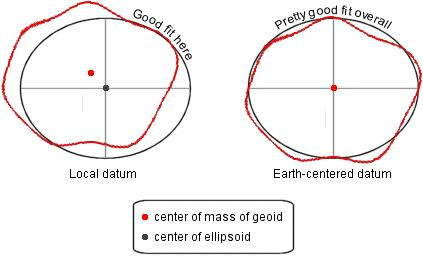
\includegraphics[width=0.75\textwidth]{pictures/datum_geotik_lokal.jpg}
		\caption{Datum geodetik lokal (Sumber : Map Projections and Coordinate Systems 2014)}
		\label{Datum geodetik loka}
		\end{figure}	

\item Datum referensi geodetik regional ellipsoid adalah dengan menggunakan bentuk yang paling sesuai dengan bentuk permukaan geoid ke area yang relatif lebih luas dari datum lokal. Datum regional biasanya dibagi oleh Negara yang berdekatan dengan negara yang terletak di satu benua. Contohnya termasuk: datum datum regional dan datum NAD Indian (North-American Datum) 1983 yang merupakan datum untuk negara-negara yang terletak di bagian utara Amerika, Eurepean 1989 Datum digunakan oleh negara negara yang terletak di benua Eropa, dan Australia Datum Geodetik digunakan pada tahun 1998 yang terletak di benua Australia.
\begin{figure}[htbp]
		\centering
		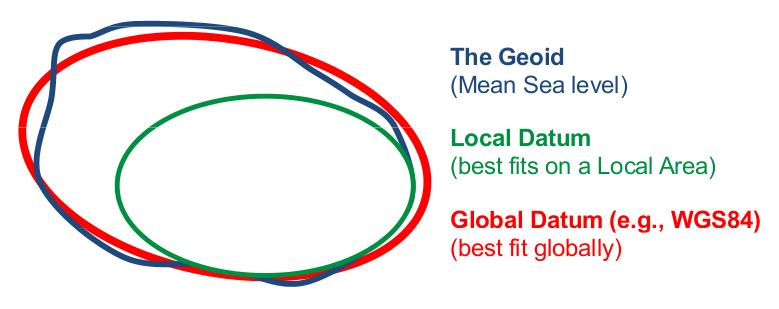
\includegraphics[width=0.75\textwidth]{pictures/datum_referensi_geodetik_regional_ellipsoid.jpg}
		\caption{Datum referensi geodetik regional ellipsoid (Sumber : Nauipedia)}
		\label{Datum referensi geodetik regional ellipsoid}
		\end{figure}	

\item Global Datum datum geodetik adalah referensi ellipsoid untuk digunakan sesuai dengan bentuk geoid dari seluruh permukaaan Bumi. Karena penggunaan datum yang berbeda di negara yang berdekatan serta karena perkembangan teknologi positioning yang sedang mengalami kemajuan pesat, maka penggunaan datum menunjuk ke datum global. Datum datum global pertama adalah WGS 60, WGS66, WGS 72, pada awal tahun 1984 mulai digunakannya datum WGS 84, ITRF dan (Sistem Referensi Terestrial Internasional).
\end{enumerate}

\subsection{Pengertian WGS 84}
World Geodetic System adalah standar untuk digunakan dalam kartografi, geodesi, dan navigasi. Terdiri dari kerangka koordinat standar untuk Bumi, permukaan referensi standar bulat (datum atau referensi ellipsoid) untuk data ketinggian mentah, dan gravitasi permukaan ekuipotensial (geoid) yang mendefinisikan permukaan laut nominal. 
Revisi terakhir adalah WGS 84 (berasal dari tahun 1984 dan terakhir direvisi pada 2004), yang berlaku hingga sekitar 2010. Skema sebelumnya termasuk WGS 72, WGS 66, dan WGS 60. Sistem referensi koordinat WGS 84 digunakan oleh Sistem Pemosisian Global.

